\documentclass[upright, contnum]{lib/umemoria}

\depto{CIENCIAS DE LA COMPUTACIÓN}
\author{PABLO IGNACIO ESTEFO CARRASCO}
\title{REESTRUCTURACIÓN Y REFACTORIZACIÓN DE UNIT TESTS CON TESTSURGEON}
%\auspicio{.}
\date{JULIO 2013}
\guia{ALEXANDRE BERGEL}
\carrera{INGENIERO CIVIL EN COMPUTACIÓN}
\comision{ROMAIN ROBBES}{JOSÉ PINO URTUBIA}{\ }

%\usepackage{lipsum}

%\usepackage[latin1]{inputenc}
%\usepackage[T1]{fontenc}
% Niveles de produndidad para mostrar
\setcounter{secnumdepth}{4}
\setcounter{tocdepth}{4}
\usepackage{float} %== Imagenes


\begin{document}

\frontmatter
\maketitle

%% Preliminary
\begin{abstract}

% Problema
\par Actualmente la actividad de Testing es fundamental dentro del ciclo de desarrollo de cualquier proyecto de software serio. Es más, las metodologías ágiles elevan su relevancia dentro de la construcción del software a tal nivel que está prohibido añadir una nueva funcionalidad sin que se haya escrito previamente un test que la valide.

% Relevancia
\par A medida que el software crece en funcionalidades y cambian los requerimientos se vuelve más complejo. Es por eso que existen varias técnicas para reestructurar el código haciéndolo más flexible a los cambios y permitiendo que crezca. 

\par Sin embargo, los test también crecen en número y en complejidad. Por lo que no son raros los casos de test redundantes tanto desde el punto de vista de su código fuente (duplicación de test) como de su ejecución. Pero a diferencia con el código ``funcional'', poco esfuerzo se ha realizado por parte de la industria por promover técnicas y crear herramientas que faciliten la tarea de mantener su estructura y diseño limpio. 

\par Una de las consecuencias importantes de este problema, es el gran tiempo que toma ejecutar todos los tests. Al haber redundancia, la ejecución tarda más tiempo del necesario lo hace que los desarrolladores los corran con menos frecuencia e inclusive invierten menos tiempo en escribir nuevos test lo cual minimiza la cobertura. Esto último atenta críticamente en la confiabilidad del código base y por ende de la aplicación.

\par En este trabajo se propone una herramienta para detectar problemas de diseño de los tests. \emph{TestSurgeon} aborda este problema desde dos perspectivas de análisis principales: su código fuente y su ejecución. A través de una intuitiva interfaz, el desarrollador puede navegar sobre las pruebas unitarias y realizar comparaciones entre tests guiado por métricas dedicadas que facilitan la detección de casos interesantes. Además provee una completa visualización que condensa dos métricas que describen y  diferencian la ejecución de los test en comparación, permitiendo realizar un análisis eficaz. Finalmente, TestSurgeon permite detectar diferencias semánticas entre tests y encontrar redundancias entre estos para una posible refactorización.

%\par Se presenta también en detalle una experiencia de la aplicación de \emph{TestSurgeon} sobre los tests de \emph{Roassal}, un motor de visualización ágil. Se detallan tres escenarios de refactorización y reestructuración de test que la herramienta permite detectar.  
\par Se presentan distintos escenarios de refactorización y restructuración que son detectados por TestSurgeon. Estos son descritos con ejemplos reales en base a una experiencia de aplicación de \emph{TestSurgeon} sobre los tests de \emph{Roassal}, un motor de visualización ágil.   

\par \emph{TestSurgeon} ganó el primer lugar en la competencia internacional \emph{ACM Student Research Competition} (categoría pregrado) durante la conferencia ICSE (principal en Ingeniería de Software) el año 2012.

% Este problema es particularmente importante cuando se automatiza el proceso de liberación de código a través de integración contínua. Donde antes de liberar una nueva funcionalidad se ejecutan todos los tests para verificar que no se ha roto ninguna funcionalidad previamente liberada. Por tanto, el tener tests redundantes tiempo valioso se pierde y provoca disminución en la velocidad del equipo de desarrollo.  





\end{abstract}
% \begin{dedicatoria}
Por mi y por todos mis compañeros.
\end{dedicatoria}
% \begin{thanks}
Vale cabros :D
\end{thanks}

%\cleardoublepage
\tableofcontents
%\cleardoublepage
\listoftables
%\cleardoublepage
\listoffigures

\mainmatter

%% Chapters
\chapter{Introducción} 
%% Intro
\par El Testing es una actividad importante en el desarrollo de los proyectos de software en nuestro días. Los tests automatizados ayudan al desarrollador a asegurar calidad en su código y a detectar posibles \emph{bugs} o defectos en la aplicación. Más aún, los tests pueden también ser considerados como  una ``documentación ejecutable'', evitan tiempo de depuración, y pueden ser utilizados también como una primera aproximación a entender código ajeno.

\par Dada la naturaleza de las pruebas de software, su estudio e investigación se ha focalizado en mejorar su efectividad para hacer software cada vez más confiables y robustos. Al igual que el software funcional, los tests son parte del código fuente de la aplicación. La comunidad de ingeniería de software ha desarrollado diversas técnicas y metodologías para mantener limpio el diseño del código base (o funcional). Sin embargo, poco trabajo se ha realizado para que  el código de los tests mantenga una estructura y diseño limpios. Situación que pasa a ser cada vez más problemática a medida que el software crece en tamaño y en complejidad.


%% Terminologia
\section{Terminología}

\par Para la lectura adecuada del documento, se presenta la siguiente terminología con los conceptos principales que se utilizarán a lo largo del documento:

\begin{description}
\item[\emph{test}]: Corresponde a un trozo de código que tiene como finalidad simular un comportamiento particular de alguna componente o componentes del sistema para realizar verificaciones que validen el comportamiento esperado de estas. También se le nombra: \emph{método de test}, \emph{test method} o \emph{prueba de software}.
\item[\emph{unit test}]: Corresponde a un grupo de tests que, en conjunto, verifican una funcionalidad en común. También se le nombra: \emph{prueba unitaria} o \emph{grupo de tests}.
\item[\emph{smell}]: Se refiere a una deficiencia en el diseño del código que da pie a problemas en su mantenibilidad y/o extensibilidad. Cuando existen \emph{smells} sobre el código se pruebas se nombra como un \emph{test smell}.
\end{description}

%% Motivacion (pq toi haciendo esto?)
\section{Motivación}
% - Contexto: Práctica de Testing, Unit Testing
\par Actualmente el \emph{testing} es una actividad clave dentro del desarrollo de cualquier proyecto de software serio. De hecho, las metodologías ágiles de desarrollo consideran la creación de tests como el punto de partida de la iteración o ciclo de desarrollo. Ejemplos de estas son: Test-Driven Development (TDD) y Behavior-Driven Development (BDD). El escribir tests que describen la funcionalidad esperada de una unidad de software (TDD) y/o el comportamiento esperado de un conjunto de unidades (BDD), son formas de producir código confiable, puesto que no se agrega otra funcionalidad sino hasta que existe un test que lo simula y describe su funcionamiento esperado.

\par A medida que el software crece en complejidad y tamaño, de igual manera el código se va volviendo más complejo, lo cual atenta contra el crecimiento del proyecto. Para esto, la industria y la academia han desarrollado diversas formas de reestructurar y/o refactorizar el código base para enfrentar el \emph{cambio} de la forma menos costosa. Sin embargo esto no ha sido igual para el código que corresponde a los tests. A medida que el sistema evoluciona los tests necesitan hacerlo también para mantenerse actualizados con el sistema~\cite{reichhart2007rule}.  Pero muchas veces esto no sucede, los tests carecen del mismo cuidado que el código base por lo cual se hace necesario reescribir los tests. Es más, no es raro que se deje de escribir tests por el costo en tiempo que esto implica.

\par Por otro lado, la aplicación estricta de estas metodologías ágiles incrementa rápidamente la cantidad de tests. Y estos pueden clasificarse como: de bajo o alto nivel. Los  tests de bajo nivel prueban las unidades fundamentales del sistema,  mientras que los de alto nivel testean la interacción entre estas. Esto significa que al ejecutar tests de alto nivel, implícitamente se está siendo redundante con respecto a los de bajo nivel ya que está testeando una pieza de código que fue previamente ejecutada por uno o más tests de bajo nivel. Y esto puede repetirse en varios tests de alto nivel.

\par Esta redundancia representa un costo en tiempo que en algunos casos puede ser considerable, teniendo en cuenta que los tests se ejecutan frecuentemente cada vez que se agrega o modifica el código. 

\par Bajo este escenario, se hace necesaria una forma de reducir esta brecha entre el código base y el código de test, y facilitar la detección de \emph{test smells} que significan un gran costo tanto para los desarrolladores como el cliente.


\newpage
%% Objetivos
\section{Objetivos}
\par El objetivo general de este trabajo es desarrollar una herramienta que permita a los programadores refactorizar y reestructurar sus tests de una manera más fácil, segura y que considere la versatilidad de su uso.

\subsection*{Objetivos Específicos}
\begin{enumerate}
\item Identificación de las métricas relevantes para caracterización de tests methods desde el punto de vista de un análisis dinámico
\item Desarrollar una visualización que permita detectar redundancia y solapamiento entre grupos de test methods (o unit tests)
\item Investigar refactorizaciones automáticas y semi-automáticas para unit tests y sus implicancias el rendimiento y cobertura
\item Desarrollar una interfaz gráfica efectiva y usable para el uso cotidiano dentro del desarrollo de software
\end{enumerate}

%% Organizacion del documento
\section{Estructura del documento}

\par En el \chapref{espec-prob} se presenta el problema de la mantenibilidad de tests en detalle, su contexto y relevancia. En el capítulo siguiente, un marco teórico entrega los conceptos técnicos necesarios (\secref{marco-teorico}), y se presenta una serie de antecedentes que muestra el trabajo realizado tanto por la academia como por la industria sobre el problema de diseño del código de tests (\secref{trabajo-relacionado}). A continuación se presentan dos estudios (\secref{exp-static-vs-dynamic} y \secref{pq-cobertura}) realizados durante el desarrollo de esta memoria que revelan aspectos no estudiados del problema. El aprendizaje obtenido y las conclusiones de éstos determinaron varias decisiones de diseño de la solución. 

\par Luego, con la base conceptual y contextual del problema presente, se describe en detalle la solución propuesta: \emph{TestSurgeon}. Primero en forma conceptual en el \chapref{descripcion-solucion} y después en forma técnica, su implementación, en el \chapref{implementacion}. Junto con esto, en el \chapref{caso-de-estudio} se muestra una aplicación de la herramienta sobre las pruebas unitarias de un software no-trivial. 

\par Finalmente en el \chapref{conclusion} se revisa el cumplimiento de los objetivos planteados, las conclusiones del trabajo, así como también algunas directrices para continuarlo.

\par Se adjuntan además algunos apéndices que complementan el documento y entregan datos que por su extensión no pudieron ser incluidos directamente en los capítulos.

\chapter{Especificación del Problema}\chaplabel{espec-prob}
% Conceptos para que el lector entienda y pueda leer depsués



\section{Contexto: Test como ``conductores'' del diseño}
\par Durante el desarrollo de un software una de las actividades principales es el testeo de los requerimientos. Existen variadas técnicas, metodologías y artefactos relacionados a esta actividad. En particular, la creación de pruebas automatizadas es una práctica cotidiana en cualquier proyecto de software y comprende parte importante de los artefactos generados. \\

\par En particular los proyectos de software ágiles dan gran importancia a estos artefactos, ya que cada historia de usuario (requerimiento) debe tener pruebas de aceptación (tests de alto nivel). Estos se escriben y detallan en conjunto con el cliente para asegurar que el código que se creará cumple lo que este pide: ni menos ni más.

\par Estas historias de usuario están escritas en lenguaje natural por lo que se deben \emph{transcribir} al lenguaje técnico: código fuente. Entonces, antes de escribir una funcionalidad, los desarrolladores crean los tests: código fuente que garantiza que una característica se comporta como es requerida. Este proceso se denomina \emph{Test-Driven Development} (o TDD)~\cite{Beck02a}  o Desarrollo Dirigido por Pruebas: se escribe el test, se ejecuta y este falla (ya que no se ha escrito el código que suple dicha característica). Luego se escriben las clases y métodos que hace el test funcionar, éste se vuelve a ejecutar y esta vez ``pasa''. Finalmente se refactoriza el código recién escrito para mantener un diseño limpio y mantenible en el tiempo.

\par Esta práctica está dentro del núcleo de la filosofía que enmarca la agilidad a tal nivel que está prohibido agregar una nueva funcionalidad sin, previamente, haber escrito un test que lo valide~\cite{Beck02a}. Esta queda documentado en el libro de Robert Cecil Martin (más conocido como``Uncle Bob'')~\cite{Mart02b} uno de los escritores del manifiesto ágil~\cite{Fowl01a} quien declara:

\begin{quote}
\emph{``The iteration between writing test cases and code is very rapid [...]. As a result, a very complete body of test cases grows along with the code.''}
\end{quote}


\par En la práctica, aplicando TDD se obtiene una gran cantidad de pruebas unitarias (unit tests) que representan los casos de prueba de la aplicación (Test Cases). Cada Unit Test contiene varios métodos de tests (test methods) que cubren los distintos aspectos a verificar en la funcionalidad que se está testeando.


\section{Problema: ¿Cómo mantener los tests?}

\par La comunidad de ingeniería de software ha producido herramientas efectivas y buenas prácticas para lograr refactorizaciones en el código base que otorguen un buen diseño. Sin embargo, en cuanto al código de las pruebas de software no sucede en igual proporción. Es más, éstos son raramente modificados y carecen del cuidado que se le da al código base, sin pensar su modularidad ni extensibilidad. 

\par Por lo cual no es difícil encontrar deficiencias como \textbf{solapamientos} entre test methods o más general, entre test cases. Estos solapamientos pueden ser de carácter estático ( duplicación de código ), o bien dinámicos, es decir que dos test methods tienen ejecuciones similares y por consiguiente representan una ineficiencia de tiempo.

\par Estas deficiencias en el diseño y calidad del código de las pruebas unitarias tienen consecuencias importantes en la calidad del código testeado y en el mismo proceso de desarrollo:
\begin{itemize}
\item \textbf{Performance} Debido a los solapamientos previamente mencionados, muchas veces existe \textbf{ejecución redundante} que va en contra de las características deseables de una suite de tests. Muchas veces los tests dejan de ejecutarse con la frecuencia necesaria.
\item \textbf{Debugging} Otra deficiencia conocida es que al correr los tests en presencia de un \emph{bug}, éste queda en evidencia por muchos tests, lo cual dificulta la identificación de su causa y su corrección. Coloquialmente se hace más difícil responder la pregunta: \emph{¿Cuál test miro primero?}
\end{itemize}
 
\par De esta manera la confiabilidad en el producto y su calidad se ven impactadas negativamente. 

\par Un caso muy claro de la influencia del mal diseño y poco cuidado en los tests ocurre cuando el ciclo de desarrollo utiliza mecanismos de \textbf{Integración Contínua} (Continuous Integration). En esta práctica cada \emph{feature} se implementa tan pronto como es posible, se testea y se pasa a producción de inmediato. De esta manera el equipo de desarrollo realiza varias integraciones por día y el cliente obtiene rápidamente las nuevas funcionalidades a medida que las solicita. \\

\par A modo de ejemplo, la empresa MediaGeniX\footnote{MediaGeniX [en línea] \textless\url{http://www.mediagenix.tv}\textgreater [Consulta: 12/08/2013]} realiza la integración continua desde hace algunos años. Ahí, 30 desarrolladores trabajan sobre el mismo producto y cada uno de ellos construye varias versiones al día. Cada versión que se va a pasar a producción debe pasar su suite de pruebas que comprende alrededor de 30.000 tests. Ellos realizan 3 integraciones diarias en promedio, por lo cual recurren a técnicas de paralelización de ejecución de tests para lograrlo. Esto introduce un alto costo económico asociado al los recursos de hardware(servidores, clusters) y además un alto costo en tiempo. Esto se podría optimizar detectando redundancia en la ejecución. \\

% \par Esto evidencia la relevancia de mejorar la performance mediante la refactorización y restructuración de los unit tests.

\chapter{Antecedentes}


\section{Marco Teórico}\seclabel{marco-teorico}

\subsection{Profiling}

\par El \emph{Perfil de Ejecución} (o \emph{Execution Profiling}) es una forma de análisis dinámico que consiste en monitorear un software durante su ejecución para posteriormente analizar los datos obtenidos. Entonces los \emph{Profilers} son herramientas para ayudar a los ingenieros de software a recolectar datos durante la ejecución y analizarlos, y así poder determinar de mejor manera en qué parte de un sistema de software se gasta el tiempo de ejecución.


\par Para la obtención de datos, existen varias técnicas de profiling. Los principales son profiling por instrumentación (o \emph{Instrumentation-based profiling}) y a través de muestras (o \emph{Sampling-based profiling}). En la primera, se inserta código de instrumentación antes (instrumentación estática) o durante la ejecución (instrumentación dinámica). En la primera se agrega el código justo antes de ejecutar y por tanto la sobrecarga (o overhead) es menor. Sin embargo, cualquier código generado dinámicamente no será instrumentado. En tanto, la técnica basada en muestras aproxima el tiempo que se gastó en un método de la aplicación deteniendo el programa y guardando la colección de metodos que fueron ejecutados.

\par Usualmente los \emph{profilers} son utilizados con motivo de optimizar un sistema de software en cierto aspecto. Los datos a obtener a través de la técnica de profiling dependen completamente del problema a optimizar. Es por esto que el profiler a utilizar debe permitir la recolección de los datos necesarios con una mínima sobrecarga (o \emph{overhead}) para conseguir datos fidedignos y a la vez representativos. 

\par La herramienta de profiling escogida para en este trabajo es el framework \emph{Spy}, que utiliza la técnica de profiling basado en instrumentación del tipo dinámico. Spy está diseñado para analizar softwares en el contexto de orientación a objetos ya que se permite obtener métricas contextuales como: el número de ejecuciones de un método, cantidad de objetos instanciados de una clase, etc. Para mayor información sobre este y su implementación en \emph{TestSurgeon} ver la \secref{impl-spy}. 

\par Algunas de las aplicaciones exitosas basadas en Spy son \emph{Hapao}\footnote{Hapao [en línea] \textless\url{http://hapao.dcc.uchile.cl}\textgreater  [Consulta: 12/08/2013]}: una herramienta de cobertura de test desarrollada por Vanessa Peña y Alexandre Bergel~\cite{bergel2012increasing}, que permite gráficamente ver la cobertura de las clases y métodos contrastando la cobertura de los últimos con el grado de complejidad de éstos; y \emph{Kai}\footnote{Object Profile. Kai Profiler [en línea] \textless\url{http://www.objectprofile.com/\#/pages/products/kai/overview.html}\textgreater  [Consulta: 12/08/2013] }: un profiler que permite optimizar la ejecución de un software indicando, por ejemplo, dónde combiene incrustar una estructura de \emph{caching} para evitar redundancia de cálculo. En la \figref{hapao.png} y \figref{kai.png} se muestran capturas de pantalla de Hapao y Kai respectivamente.

\fig{h}{0.7}{hapao.png}{Ejemplo de la visualización de la cobertura de test en Hapao}
\fig{h}{0.7}{kai.png}{Diagnóstico de ejecución entregado por Kai}

\clearpage
%==========
\subsection{SUnit framework}

\par \emph{SUnit} es un framework de testing que apoya la creación de tests automatizados. SUnit es la implementación en Smalltalk del framework xUnit\footnote{la \textbf{x} se reemplaza por el lenguaje de programación, por ejemplo: jUnit para Java.} que de hecho historicamente es la primera. Las cualidades que caracterizan xUnit son:

\begin{itemize}
\item Los tests son repetibles: Cada test se puede ejecutar cuantas veces se quiera.
\item Los tests se ejecutan si necesidad intervención humana: Se puede dejar los tests ``corriendo'' durante la noche si necesidad de intervenir en su ejecución.
\item Los tests cuentan una historia: un test cubre al menos una funcionalidad del sistema. Un test entonces es un escenario que cualquier desarrollador puede leer para entender dicha funcionalidad.
\end{itemize}

\par En SUnit los tests están contenidos en clases llamadas unit tests. Los unit tests son clases que extienden o heredan de {\tt TestCase}, una de las clases arquitectónicas del framework. Los unit tests suelen nombrarse con el sufijo {\tt Test}, por ejemplo {\tt MarioBrosTest}. Los tests o test methods, por su parte se nombran con {\tt test} como prefijo, ejemplo {\tt testMarioFallDownAndLoseOneLife}.


\subsubsection{Arquitectura de \emph{SUnit}}
\par Estructuralmente, SUnit se compone de cuatro clases: {\tt TestSuite}, {\tt TestCase}, {\tt TestResource} y {\tt TestResult} como se muestra en \figref{sunit.pdf}. 
\begin{description}
\item[{\tt TestCase}] representa un unit test o una familia de test que comparten el mismo contexto. Esta clase está pensada para ser extendida por clases concretas. El contexto se especifica en el método {\tt setUp} donde las variables de instancia de cada subclase de {\tt TestCase} se inicializan y definen el contexto en el cual se ejecutará cada test. También se define el método {\tt tearDown} que es responsable de limpiar los objetos que hayan sido inicializados y modificados durante la ejecución del test para que pueden ser reinicializados por el método {\tt setUp}. Tanto {\tt setUp} como {\tt tearDown} son métodos abstractos. Entonces cada test se ejecuta de la siguiente manera:

\[ \texttt{setUp} \rightarrow \texttt{testMarioFallDownAndLoseOneLife} \rightarrow \texttt{tearDown} \]

\item[{\tt TestSuite}] contiene una colección de unit tests. Una instancia de {\tt TestSuite} está compuesto por instancias de subclases de {\tt TestCase} y {\tt TestSuite}. Las clases {\tt TestSuite} y {\tt TestCase} forman el patrón composite. 

\item[{\tt TestResult}] representa los resultados de una ejecución de {\tt TestSuite}. Contiene el número de tests que pasadon, el número de tests que fallaron y el número de errores.

\item[{\tt TestResource}] representa un recurso que es usado por un test o un conjunto de tests. Un recurso se asocia con una clase hija de {\tt TestCase} y se ejecuta automáticamente antes de la ejecución de todos los tests y una sola vez.   
\end{description}

\fig{h}{0.7}{sunit.pdf}{Las clases que representan el núcleo de \emph{SUnit}}

\subsubsection{Estructura de un test}
\par La estructura de cada test puede dividirse en dos partes: \emph{fixture} (o escenario) y \emph{assertions} (o verificaciones). En el fixture del test se crean e inicializan los objetos del escenario y se les hace interactuar a través de mensajes. No se considera parte del fixture todos los objetos inicializados y las operaciones realizadas en la ejecución del método {\tt setup}, aunque sí afectan la interacción en el fixture. Posteriormente, en el test hay una serie de validaciones o verificaciones, donde se comprueba el estado de los objetos a través de métodos verificadores heredados desde {\tt TestCase} tales como: {\tt assert:} para verificar una afirmación, {\tt deny:} para negarla, {\tt should:raise:} para verificar que una excepción en particular se lanzó, y {\tt shouldnt:raise:} para asegurar que no se lanzó cierta excepción.

\par A modo de ejemplo se muestra un código que bien podría ser un test básico del popular juego \emph{Super Mario Bros.}, donde un plomero de traje rojo va pasando por escenarios llenos de trampas y dificultades para poder llegar al castillo donde supuestamente está su princesa y rescatarla. Una de las trampas más comunes y sencillas del juego son hoyos de profundidad infinita donde Mario puede caer y perder una vida. En el ejemplo, inicializamos la variable local {\tt mario} con una instancia de la clase {\tt MBMario} que por defecto tiene 3 vidas\footnote{En la plataforma NES, Mario parte con 3 vidas.}. Luego lo insertamos al juego junto con un escenario en el cual, luego de dar tres pasos debiera caer a un hoyo y perder una vida. En el juego no se acaba sino hasta que a Mario se le acaban las vidas y vemos el mensaje de ``Game Over''. 

\begin{codeWithLineNumbers}
<i>MarioBrosTest>>testMarioFallDownAndLoseOneLife</i>
	" *--* Fixture *--* "
	| game mario scene |
	game := MBGame new.
	mario := MBMario new. " todos saben que Mario parte con 3 vidas"
	scene := #(#floor #floor #hole #floor). " un escenario con un hoyo en la tercera posicion"

	game setScene: scene.
	game setPlayer: mario.

	" hagamos a mario avanzar en el escenario"
	mario moveOneStep. 
	mario moveOneStep.
	mario moveOneStep. 
		
	" *--* Assertions *--* "
	
	self assert: (game currentPosition = #hole) "mario cayo al hoyo" 
	self assert: mario isDead. "deberia haber muerto puesto que cayo al hoyo"
	self assert: (mario lives = 2). "mario ahora tiene 2 vidas"
	self deny: game isGameOver. 
	

\end{codeWithLineNumbers}

\newpage
%=======
\section{Trabajo Relacionado}\seclabel{trabajo-relacionado}

\par A continuación se presenta una revisión de la literatura sobre el problema de mantenibilidad de las pruebas de software, y una revisión también de las herramientas de cobertura de test que abordan tangencialmente el problema.

\subsection{Revisión de la literatura}
\par Luego de revisar la bibliografía existente, entre los problemas con mayor investigación está la cobertura de los test: cómo medir y mejorar la cobertura del software testeado para aumentar la confiabilidad en éste; y  el testeo por mutación: como mejorar la efectividad de los test realizando variaciones en el código testeado que representan bugs y comprobar que test definidos atrapan o detectan esas anomalías. Con respecto al problema de mantenibilidad, las estrategias encontradas en la literatura corresponden a priorización de tests y comparación de tests, pero en volumen mucho menor a los tópicos mencionados anteriormente.

\par La priorización de tests y el \emph{clustering} son acercamientos populares para manejar el gran costo de correr una cantidad considerable de tests. Shin Yoo \etal~\cite{yoo2009clustering} han presentado un mecanismo para reducir las comparaciones 1-a-1 agruparlos y de esa manera facilitar la tarea humana de priorizar tests. Ellos crearon clusters de tests agrupándolos por similitud de ejecución. Cada ejecución fue representada por una cadena binaria donde cada dígito (1 o 0) representa si cierto método fue ejecutado durante ésta. Entonces, la similitud de cobertura es medida a través de una distancia binaria.

\par Vengala \etal~\cite{Vang09a} crearon un mecanismo para usar análisis estático y dinámico para optimizar las actividades de testing tales como \emph{selección de test}, \emph{eliminación de redundancia} y \emph{priorización de test}. Aunque sus métricas siguen el mismo espíritu que \emph{TestSurgeon}, están definidas para un ambiente de programación procedural lo cual es incompatible en un ambiente orientado a objetos.

\par Greiler \etal~\cite{Grei12a,greiler2012test} aborda el problema de entendimiento de tests suites proponiendo un framework sobre correlación entre similitud de test (Test Similarity Correlator). Este último produce una traza de ejecución que caracteriza la ejecución de los test a través de cuatro tipos de eventos: ejecución de un test method, evento de set-up y tear-down, ejecución de un método y lanzamiento de excepción. El entendimiento de test suites se realiza comparando las trazas de ejecución.

\par El código de test, desde el punto de vista de un artefacto de software tiene múltiples usos. Uno de ellos es documentación~\cite{Kuhn08a}. Especialmente para desarrolladores nuevos que tienen que enfrentarse con sistemas legados, los tests son altamente relevantes como ejemplos de código. Siguiendo esta perspectiva, Lienhard \etal~\cite{Lien08a} proponen una herramienta que facilita la tarea de escribir nuevos tests para esos sistemas a través de una visualización que llaman \emph{Test Blueprint}, como una guía para el entendimiento de los tests y el mantenimiento del código base.  

\par Reichhart \etal~\cite{reichhart2007rule} presenta \emph{TestLint}, una herramienta para determinar la calidad de los tests. En su trabajo presenta una aplicación de esta sobre una gran cantidad de unit tests obtenidos desde distintos repositorios open source. Además entrega una gran lista de \emph{test smells} de los cuales uno es analizado por \emph{TestSurgeon} y corresponde al escenario descrito en la \secref{escenario2}.

\par De los autores encontrados, el que aborda con mayor profundidad el problema de mantenibilidad en los tests es Markus Gaelli. Dentro de su investigación~\cite{gaelli2006composing,gaelli2007composing} presenta un estudio de clasificación de unit test~\cite{gaelli2005towards} representado por un arbol binario cuyas ramas indican cumplimiento de un criterio de clasificación. En este arbol, las hojas son los distintos tipos de test: Test donde se llama un solo método exactamente una sola vez(~50\% del total de tests estudiados), Test donde se llama un solo método en varios escenarios distintos (15\%), etc. Luego, utilizando esta taxonomía crea un metamodelo para escribir tests a través de ejemplos (o tests de alto nivel) a través de composiciones de tests más pequeños y de bajo nivel. Este modelo facilita la detección de errores ya que al componer tests, un bug en el código base sólo rompería uno de los tests de los que conforman el test ejecutado. Gaelli en su trabajo pretende en su trabajo promover la reutilización de tests de bajo nivel para crear ejemplos de funcionamiento, o tests de alto nivel. De esta generar ejemplos que sirven tanto como pruebas de software y documentación ejecutable~\cite{gaelli2006modeling}, acercando la brecha entre las unidades de software y las pruebas unitarias.

\subsection{Revisión de herramientas de cobertura de test existentes}

\par La gran cantidad de herramientas disponibles ilustra la importancia de la cobertura de tests para los profesionales de la industria. Se realizó una revisión de muchos de ellos incluyendo Emma, EclEmma, JCover, GroboCodeCoverage, JCoverage, Parasoft JTest, Purity Plus, Semantic Designs, TCAT, Quilt, NoUnit, InsectJ, Hansel, Gretel, Jester, JVMDI Code Coverage, JBlanket, Coverlipse, Koalog, Cobertura, Mojo y Thucydides. En el \apref{review-test-coverage-tools} se presenta la lista con las URL donde se puede obtener cada una de ellas. Esta recolección de las herramientas más populares se realizó a través de motores de búsqueda en la web, directorios de proyectos open source, descripciones de entornos de desarrollo y publicaciones científicas entre los que están: maven\footnote{Apache Maven Project [en línea] \textless\url{http://maven.apache.org/}\textgreater [Consulta: 12/08/2013]}, sourceforge\footnote{Sourceforge [en línea] \textless\url{http://sourceforge.net/}\textgreater [Consulta: 12/08/2013]}, github\footnote{GitHub [en línea] \textless\url{http://github.com/}\textgreater [Consulta: 12/08/2013]}, bitbucket\footnote{BitBucket [en línea] \textless\url{http://bitbucket.org}\textgreater [Consulta: 12/08/2013]} y el Eclipse marketplace\footnote{Eclipse Marketplace [en línea] \textless\url{http://marketplace.eclipse.org/}\textgreater [Consulta: 12/08/2013]}. 

\par Dentro de las 22 herramientas de cobertura de test estudiadas, solo 3 soportan un análisis comparativo de cobertura de test. 
\par JCover indica las variaciones de cobertura mostrando un gráfico tipo \emph{scatterplot} puntos representando los pares \emph{(version del software, \% cobertura)}. Al parecer TCAT compara tests, sin embargo no hay suficiente información publicada, de hecho, su sitio web no ha sido actualizado desde el año 2008. Jester realiza mutación a los tests para verificar cuán capaz es el unit test de capturar variaciones en el código base.


\chapter{Descripción de la Solución}
% Describir el alcance Alcance
\section{Solución}

\par Como se detalló anteriormente se desea restructurar y refactorizar los tests porque X, Y y Z.
\par Considerando el estudio comparativo entre datos estáticos y dinámicos 
Profiling pq asi se ve lo que realmente se ejecuta
Métrica

Clustering --> reducir el esfuerzo de la inspección
Visualizacion --> inspección


\section{Implementación}
\par El proyecto TestSurgeon fue completamente implementado en el lenguaje Pharo Smalltalk\emph{Pharo}\footnote{Pharo Project - \url{http://www.pharoproject.org} - última visita 12-07-2013 } ya que es en lenguaje en el que está escrito el framework de profiling utilizado. 
%Pharo es un lenguaje de programación que sigue el paradigma de orientación a objetos cuyas principales ventajas son, primero: entorno de desarrollo robusto totalmente integrado al lenguaje, y segundo: el sistema sigue una orientación a objetos pura, es decir, todo en Pharo es un objeto, Strings, Números, Clases, Métodos, Paquetes, etc. La segunda característica favorece el desarrollo de TestSurgeon en cuanto todo el modelo de lo que es un bo

\subsection{Profiling}
% http://www.bergel.eu/download/papers/Berg10f-Spy.pdf
\par La componente principal de TestSurgeon es la que realiza el profiling. Por eso se escogió una herramienta que fuera fácil de utilizar y que permitiera obtener la mayor cantidad de datos sobre la ejecución de un test.
\par El framework de profiling escogido fue \emph{Spy} y está escrito en el lenguaje Pharo. Entre sus características está que es un profiler orientado a los métodos. Considerando que en Pharo todas las interacciones corresponden a objetos que se comunican a través de mensajes, este punto es muy importante. Si se quiere conocer el comportamiento de un test con gran detalle, el hacer profiling de los métodos que son llamados durante su ejecución es fundamental. 
\par Además, Spy posee una arquitectura muy simple y fácil de extender. Consta de cuatro clases principales: {\tt Profiler}, {\tt PackageSpy}, {\tt ClassSpy} y {\tt MethodSpy}. {\tt Profiler} es la clase principal con las características necesarias para la instrumentación, ejecución y obtención de datos. Las demás clases contienen información sobre el profiling de los paquetes instrumentados y de sus clases y métodos respectivamente. 
\par La clase {\tt MethodSpy} técnicamente es un \emph{wrapper} de un método en Pharo (una instancia de la clase {\tt CompiledMethod}) que acumula datos sobre el contexto de su ejecución. Para esto, la clase provee los métodos {\tt beforeRun: with: in:} y {\tt aftefRun: with: in: } que son ejecutados justo antes e inmediatamente después de ejecutado el método instrumentado. Así se obtienen los datos del impacto de la ejecución de dicho método en el objeto y en los objetos con los cuales colabora. Estos métodos son abtractos y deben concretarse en las aplicaciones que decidan usar Spy extendiendo sus clases. 

%== Figura: Clases y extensión

\par Para hacer uso de Spy se deben entonces extender las clases antes mencionadas y acondicionarlas al dominio específico del problema. Estas clases son: {\tt TSProfiler}, {\tt TSPackage}, {\tt TSClass}, {\tt TSMethod}. Para las aplicaciones que usan esta información, se necesitan obtener datos de ejecución tanto de los tests como del código testeado, es por eso, que para representar un método de test se tiene también la clase {\tt TSTestMethod} que es un wrapper de la clase {\tt TSMethod} donde se guardan métricas y datos procesados de ésta que corresponden a un test method y no a un método testeado, como por ejemplo: {\tt testedMethods}, {\tt testedClasses} o {\tt visualizeDifferencesWith:}, entre otros.

\par A continuación se describen las clases que componen al paquete {\tt TestSurgeon-Core-Spy}:

%  ---* TSProfiler *---
\subsubsection{La clase {\tt TSProfiler}}

\par Es la clase principal, su interfaz componen los siguientes constructores {\tt buildForClassCategory:} y {\tt buildForPackagesMatching:}. En ambos, el argumento es un objeto String, en el primero especifica una categoría y en el segundo una expresión regular que representa un grupo de categorías o paquetes de software de Pharo. Luego de obtenidos la categoría o las categorías, las instrumenta creando las clases {\tt TSPackage}, {\tt TSClass} y {\tt TSMethod}, posteriormente corre los tests y finalmente retorna la instancia del profiler.

\par La instancia de {\tt TSProfiler} tiene los siguientes métodos:

\begin{description}
\item[{\tt allTestMethods}] retorna una colleción colección con instancias de la clase {\tt TSMethod} que corresponde a test methods.
\item[{\tt allTestedMethods}] retorna una colleción colección con instancias de la clase {\tt TSMethod} que corresponde a los métodos testeados.
\item[{\tt compiledToSpyMethod:}] se le pasa como argumento una instancia de la clase {\tt CompiledMethod} y retorna la instancia {\tt TSMethod} que lo encapsula.
\item[{\tt plainClasses}] retorna una colección con todas las clases instrumentadas (instancias de {\tt TSClass}) que no corresponden a unit tests.
\item[{\tt testClasses}] retorna una colección con todas las clases instrumentadas (instancias de {\tt TSClass}) que corresponden a un unit test.
\end{description}

%  ---* TSPackage & TSClass *---
\subsubsection{Las clases {\tt TSPackage} y {\tt TSClass}}

\par Estas dos clases como ya se dijo, representan a los paquetes y clases instrumentadas respectivamente. En general no se necesitó información particular de los paquetes por lo que no hay nada que comentar sobre su implementación.

\par Sobre {\tt TSClass} esta representa tanto a las clases testeadas como a lo unit tests, y posee mayoritariamente métodos de ayuda o \emph{helpers} para las distintas aplicaciones (visualización, clustering, etc) como por ejemplo: {\tt allMethodsTestedBy:} donde se le entrega un {\tt TSTestMethod} y se retorna todos los métodos definidos en su clase que son llamados durante la ejecución de ese test.  

%  ---* TSMethod  *---
\subsubsection{Las clase {\tt TSMethod} }
\par El profiling de Spy es orientado a los métodos, por tanto en esta clase es donde se registran todos los datos de la ejecución para caracterizar a los tests y poder diferenciarlos.
\par Su comportamiento está dividido en dos partes principalmente: los métodos de profiling donde se registran los datos de ejecución, y sus accesores, métodos que entregan la información obtenida. Los métodos de profiling son dos: {\tt beforeRun: with: in:} y {\tt aftefRun: with: in: } (ver código en \ref{code:before-run} y en \ref{code:after-run})

%== Codigo: \ref{code:before-run} y en \ref{code:after-run}
\begin{codeWithLineNumbers}
beforeRun: methodName with: listOfArguments in: receiver
	| testMethod |
	testMethod := self profiler class currentTestMethod.
	currentTestMethodSpy := 
			spyMethodMapping at: testMethod ifAbsentPut: 
				[ self profiler >> testMethod class name >> testMethod selector ].
		
	"Local copy of instrumented test method"	
	self addTestMethod: currentTestMethodSpy.

	"ADD RECEIVER"
	self updateReceiversWith: receiver for: currentTestMethodSpy.

	"SIDE EFFECTS"
	receiverSnapshot := receiver snapshotAsInteger.

\end{codeWithLineNumbers}\label{code:before-run} 
\caption{Ble}

\begin{codeWithLineNumbers}
afterRun: methodName with: listOfArguments in: receiver

	"Count if it was a change in the receiver state"
	(receiver snapshotAsInteger ~= receiverSnapshot) ifTrue: [self plusOneIn: stateChanges at: currentTestMethodSpy ]. 

	currentTestMethodSpy := nil.
	receiverSnapshot := nil.

\end{codeWithLineNumbers}\label{code:after-run}
\lstlistingname


%  ---* TSTestMethod  *---
\subsubsection{Las clase {\tt TSTestMethod} }

\subsection{Visualización}

\subsection{Clustering}

\subsection{Browser}


\par Todo el código detallado en las secciones anteriores está almacenado en el sitio \emph{SmalltalkHub}\footnote{Smalltalk Hub - \url{http://www.smalltalkhub.com} - última visita 12-07-2013 } el repositorio ubicado en la siguiente dirección: \url{smalltalkhub.com/#!/~PabloEstefo/TestSurgeon/}. 
\chapter{Implementación}
% +-- TODO --*
% - Figura:
%	- Diagrama de clases por cada paquete
% - Hablar de spec
% - Referencias:
% 	- http://www.bergel.eu/download/papers/Berg10f-Spy.pdf (presentacion Spy)


%=======
\section{Arquitectura}\seclabel{impl-arq}

\par El proyecto TestSurgeon fue completamente implementado en el lenguaje Pharo Smalltalk\footnote{Pharo Project - \url{http://www.pharoproject.org} - última visita 12-07-2013 } ya que es en lenguaje en el que está escrito el framework de profiling utilizado (componente principal del proyecto). Pharo es un lenguaje de programación que implementa fielmente el paradigma de orientación a objetos. Sus características principales son, primero: entorno de desarrollo robusto totalmente integrado al lenguaje, y segundo: el sistema sigue una orientación a objetos pura, es decir, todo en Pharo es un objeto, Strings, Números, Clases, Métodos, Collecciones, Paquetes, etc. 

\par Para ejecutar Pharo, es necesario una máquina virtual la cual es específica de cáda sistema operativo y actúa como interfaz de este último. La imagen de Pharo, una {\tt snapshot} del sistema Pharo congelado en el tiempo, específicamente de la última vez que se ejecutó. Contiene todas las instancias creadas y en el estado en que estaban justo antes de que la máquina virtual se cerrara.

\par Sobre Pharo están: \emph{Spy}, \emph{Roassal} y \emph{Spec}, las principales dependencias de TestSurgeon. \emph{Spy} es un framework de profiling usado en TestSurgeon, se comentará en detalle sobre éste en la \secref{impl-spy}. \emph{Roassal} es un software que permite desarrollar visualizaciones interactivas en forma fácil y rápida. Es usado por TestSurgeon para implementar la \emph{Test Difference blueprint} (ver \secref{test-diff-blueprint}), en la \secref{impl-viz} se hablará de esta. Finalmente \emph{Spec} .% - Hablar de spec

\fig{H}{0.7}{impl/arq.pdf}{Arquitectura de \emph{TestSurgeon}}


%=======
\section{Profiling}\seclabel{impl-spy}
 
\par La componente principal de TestSurgeon es la que realiza el profiling. Por eso se escogió una herramienta que fuera fácil de utilizar y que permitiera obtener la mayor cantidad de datos sobre la ejecución de un test.
\par El framework de profiling escogido fue \emph{Spy} y está escrito en el lenguaje Pharo. Entre sus características está que es un profiler orientado a los métodos. Considerando que en Pharo todas las interacciones corresponden a objetos que se comunican a través de mensajes, este punto es muy importante. Si se quiere conocer el comportamiento de un test con gran detalle, el hacer profiling de los métodos que son llamados durante su ejecución es fundamental. 

\par Además, Spy posee una arquitectura muy simple y fácil de extender. Consta de cuatro clases principales: {\tt Profiler}, {\tt PackageSpy}, {\tt ClassSpy} y {\tt MethodSpy}. {\tt Profiler} es la clase principal con las características necesarias para la instrumentación, ejecución y obtención de datos. Las demás clases contienen información sobre el profiling de los paquetes instrumentados y de sus clases y métodos respectivamente. 

\par La clase {\tt MethodSpy} técnicamente es un \emph{wrapper} de un método en Pharo (una instancia de la clase {\tt CompiledMethod}) que acumula datos sobre el contexto de su ejecución. Para esto, la clase provee los métodos {\tt beforeRun: with: in:} y {\tt aftefRun: with: in: } que son ejecutados justo antes e inmediatamente después de ejecutado el método instrumentado. Así se obtienen los datos del impacto de la ejecución de dicho método en el objeto y en los objetos con los cuales colabora. Estos métodos son abtractos y deben concretarse en las aplicaciones que decidan usar Spy extendiendo sus clases. 

%== Figura: (UML) Clases y extensión
\fig{H}{0.95}{impl/spy-testsurgeon.pdf}{Diagrama de clases de {\tt Spy-Core} y {\tt TestSurgeon-Core-Spy}}


\par Para hacer uso de Spy se deben entonces extender las clases antes mencionadas y acondicionarlas al dominio específico del problema. Estas clases son: {\tt TSProfiler}, {\tt TSPackage}, {\tt TSClass}, {\tt TSMethod}. Para las aplicaciones que usan esta información, se necesitan obtener datos de ejecución tanto de los tests como del código testeado, es por eso, que para representar un método de test se tiene también la clase {\tt TSTestMethod} que es un wrapper de la clase {\tt TSMethod} donde se guardan métricas y datos procesados de ésta que corresponden a un test method y no a un método testeado, como por ejemplo: {\tt testedMethods}, {\tt testedClasses} o {\tt visualizeDifferencesWith:}, entre otros.

\par En el resto de la sección se describe en detalle las clases que componen al paquete {\tt TestSurgeon-Core-Spy}.

%  ---* TSProfiler *---
\subsection{La clase {\tt TSProfiler}}

\par Es la clase principal, su interfaz componen los siguientes constructores {\tt buildForClassCategory:} y {\tt buildForPackagesMatching:}. En ambos, el argumento es un objeto String, en el primero especifica una categoría y en el segundo una expresión regular que representa un grupo de categorías o paquetes de software de Pharo. Luego de obtenidos la categoría o las categorías, las instrumenta creando las clases {\tt TSPackage}, {\tt TSClass} y {\tt TSMethod}, posteriormente corre los tests y finalmente retorna la instancia del profiler.

\par La instancia de {\tt TSProfiler} tiene los siguientes métodos:

\begin{table}[h] 
    \centering 
    \begin{tabular}{|l|l|}
    	\hline
Selector & Resultado \\ \hline \hline
{\tt allTestMethods}	& retorna una colleción de todos los tests ejecutados (instancias\\
						&  de {\tt TSMethod}  \\ \hline
{\tt allTestedMethods} & retorna una colleción de todos los métodos testeados (instancias  \\
						& de {\tt TSMethod} \\ \hline
{\tt compiledToSpyMethod:} & encapsula un método compilado (instancia de {\tt CompiledMethod}) \\
						& retornándolo como instancia de {\tt TSMethod} . \\ \hline
{\tt plainClasses} & retorna una colección con todas las clases instrumentadas (instancias de  \\ 
						&{\tt TSClass}) que no corresponden a unit tests. \\ \hline
{\tt testClasses} & retorna una colección con todas las clases instrumentadas (instancias de \\ 
						&{\tt TSClass}) que corresponden a un unit test. \\ \hline
    \end{tabular}
    \caption{API pública de las instancias de {\tt TSProfiler}}
    \tablabel{impl-tsprofiler}
\end{table} 


%  ---* TSPackage & TSClass *---
\subsection{Las clases {\tt TSPackage} y {\tt TSClass}}

\par Estas dos clases, representan a los paquetes y clases instrumentadas respectivamente. En general no se necesitó información particular de los paquetes por lo que no hay nada que comentar sobre la implementación de {\tt TSPackage}.

\par Sobre {\tt TSClass} esta representa tanto a las clases testeadas como a lo unit tests, y posee mayoritariamente métodos de ayuda o \emph{helpers} para las distintas aplicaciones (visualización, clustering, etc) como por ejemplo: {\tt allMethodsTestedBy:} donde se le entrega un {\tt TSTestMethod} y se retorna todos los métodos definidos en su clase que son llamados durante la ejecución de ese test.  

%  ---* TSMethod  *---
\subsection{Las clase {\tt TSMethod} }
\par El profiling de Spy es orientado a los métodos, por tanto en esta clase es donde se registran todos los datos de la ejecución para caracterizar a los tests y poder diferenciarlos. Cada instancia de {\tt TSMethod} representa un método ejecutado, es decir, tanto el test que comienza la ejecución como todos los métodos llamados durante esta. Los datos son almacenados en variables de instancia, y existe solo una instancia por método definido en el software a analizar, entonces, un método ejecutado tendrá la información sobre su ejecución en distintos tests donde haya sido llamado. Las variables de instancia se definen a continuación:

\begin{table}[h] 
    \centering 
    \begin{tabular}{|l|l|}
    	\hline
Atributo & Descripción \\ \hline \hline
{\tt testedBy}	& Diccionario que asocia cada test con las veces que el \\
				& método fue llamado por éste durante la ejecución del primero\\ \hline
{\tt originalMethod} & instancia de {\tt CompiledMethod} correspondiente al  \\
						& método encapsulado. \\ \hline
{\tt receiverFootprintsMapping} & Diccionario que asocia un test con todos los objetos \\
						& \emph{receivers} del método actual durante su ejecución. \\ \hline
    \end{tabular}
    \caption{Atributos principales de {\tt TSMethod}}
    \tablabel{impl-tsmethod}
\end{table} 

\par Su comportamiento está dividido en dos partes principalmente: los métodos de profiling donde se registran los datos de ejecución, y sus accesores, métodos que entregan la información obtenida. Los métodos de profiling son dos: {\tt beforeRun: with: in:} y {\tt aftefRun: with: in: }, a continuación se muestra el código del primero. 

%== Codigo: \ref{code:before-run} y en \ref{code:after-run}
\begin{codeWithLineNumbers}
<i>beforeRun:</i> methodName <i>with:</i> listOfArguments <i>in:</i> receiver
	| testMethod |
	" Test en ejecucion "
	testMethod := self profiler class currentTestMethod.
	currentTestMethodSpy := 
			spyMethodMapping at: testMethod ifAbsentPut: 
				[ self profiler >> testMethod class name >> testMethod selector ].
		
	" Guardar en el diccionario de tests"	
	self addTestMethod: currentTestMethodSpy.

	" Guardar receiver "
	self updateReceiversWith: receiver for: currentTestMethodSpy.

\end{codeWithLineNumbers}\label{code:before-run} 

\par Los dos métodos señalados son ejecutados por todos los métodos dentro de la ejecución del test, incluso este último. Sin embargo, la estrategia de obtención de los datos de ejecución es que los métodos instrumentados del código base sean los que almacenen los datos de esta. 

\par En el código de {\tt beforeRun:with:in:}, una instancia de {\tt TSMethod} lo recibe. Lo primero que realiza es obtener el test que originó la ejecución. Para esto, realiza un llamado al profiler para solicitar el test que se está ejecutando en ese moomento. El test se agrega al diccionario {\tt spyMethodMapping} que representa una biyección entre los tests como {\tt CompiledMethod} y su método Spy que lo encapsula. 

\par Posteriormente, el test encapsulado se agrega como llave a {\tt testedBy} (diccionario de tests que cada método del código base posee) y se incrementa en 1 el contador. También se agrega el objeto está ejecutando el método a la lista de \emph{receivers} para el test en ejecución. En el diccionario {\tt receiverFootprintsMapping}, se asocia el test y se agrega el valor de hash del objeto receptor a la colleción de receivers para ese test.

\par Las instancias de {\tt TSMethod} son entonces las principales fuentes de datos para la creación de métricas y visualizaciones. Para esto cuenta una API pública que se detalla a continuación:  

\begin{table}[h] 
    \centering 
    \begin{tabular}{|l|l|}
    	\hline
Selector & Resultado \\ \hline \hline

{\tt numberOfCallsFrom: } & Retorna el valor de la métrica \emph{Number of Calls}\\
						& (o {\tt NOC}, ver \secref{viz-metricas}). \\ \hline
{\tt numberOfReceiversDuringExecutionOf:} & Retorna el valor de la métrica \emph{Number of Different}  \\ 
						&\emph{Receivers} (o {\tt NODR}, ver \secref{viz-metricas}). \\ \hline
{\tt differencesBetweenNoCFrom:and:}	& Retorna la diferencia entre la métrica {\tt NOC} entre\\
						&  dos tests. \\ \hline
{\tt differencesBetweenNoDRFrom:and:} & Retorna la diferencia entre la métrica {\tt NODR}  entre\\
						&  dos tests. \\ \hline
{\tt numberOfTestMethodsThatCallIt} & Retorna el número de tests en los cuales es  \\ 
						& ejecutado.\\ \hline
{\tt unitTestThatTestsIt} & Retorna el número total de unit tests donde algún  \\ 
						& test haya lo ejecutado. \\ \hline						
    \end{tabular}
    \caption{API pública de las instancias de {\tt TSMethod}}
    \tablabel{impl-tsmethod2}
\end{table} 


%  ---* TSTestMethod  *---
\subsection{Las clase {\tt TSTestMethod} }
\par Como se explicó anteriormente, las instancias de {\tt TSMethod} pueden encapsular un método compilado del código base o bien de los tests que inician la ejecución de éstos. La API pública presentada anteriormente está enfocada a consultas para métodos del código base. Para el análisis de los tests es necesario incluírlos también como entidades del modelo de clases. Para eso está {\tt TSTestMethod} que básicamente es un \emph{wrapper} de una instancia {\tt TSMethod} que encapsula un test method.

\par A continuación se presenta su API pública: 

\begin{table}[h] 
    \centering 
    \begin{tabular}{|l|l|}
    	\hline
Selector & Resultado \\ \hline \hline

{\tt numberOfTestedMethods } & Retorna el número de métodos testeados.\\ \hline
{\tt testedClasses} & Retorna una colección con las clases ({\tt TSClass}) que \\ 
						& contengan métodos testeados.\\ \hline
{\tt testedMethods}	& Retorna una colección con los métodos ({\tt TSMethod}) \\
						& testeados. \\ \hline
{\tt visualizeDifferencesWith:} & Retorna una instancia {\tt TSTestDifferenceBlueprint},\\
						&  la visualización comparativa con el test entregado\\
						&  como argumento. \\ \hline
{\tt compareWith:} & Retorna una instancia {\tt TSDynCoverageOtoOComp}, \\  
						&  un comparador 1-a-1  de test que provee métricas \\
						&  de similitud dinámica.\\ \hline		
{\tt staticCompareWith:} & Retorna una instancia {\tt TSStaticOtoOComp},  \\ 
						& un comparador 1-a-1 de test que provee métricas \\
						& de similitud estática.\\ \hline						
    \end{tabular}
    \caption{API pública de las instancias de {\tt TSTestMethod}}
    \tablabel{impl-tstestmethod}
\end{table} 



%=======
\section{Visualización}\seclabel{impl-viz}
%% Method Shape: hablar del ajuste logaritmico.
\par La implementación de \emph{Test Difference Blueprint} es la clase {\tt TSTestDifferenceBlueprint}. Para crear la visualización necesita de los datos de los tests a comparar, por lo cual dentro de sus atributos están {\tt redTest} y {\tt blueTest}, instancias de {\tt TSTestMethod}. Además, posee un comparador de similitud dinámica el cual está almacenado en el atributo {\tt comparator}. Para la información general sobre toda la instrumentación y ejecución es que se necesita una instancia de {\tt TSProfiler} la cual está referenciada por el atributo {\tt profiler}. 

\par La visualización como tal corresponde instancia de la {\tt ROView}, que es básicamente un contenedor de los elementos gráficos y es responsable de mostrarlos apropiadamente. Por otro lado, enviando el mensaje {\tt exportAs:}, el objeto crea un archivo de imagen vectorial (formato {\tt SVG}) con el {\tt String} entregado como parámetro como nombre. Técnicamente no hay más aspectos destacables que no se puedan apreciar en forma directa desde el código fuente. Más información sobre la visualización se puede encontrar en la \secref{test-diff-blueprint}. 

%=======
\section{Browser}\seclabel{impl-browser}
%http://hal.inria.fr/docs/00/70/80/67/PDF/SpecTechReport.pdf
\par El browser o navegador permite acceder rápidamente a los métodos a través de menúes que permiten seleccionar unit tests y los tests para realizar comparaciones rápidamente.  Esta interfaz está implementada completamente usando el framework Spec, y gráficamente consiste en cuatro espacios: Selector de Unit Tests, Selector de Test methods, Zona de Visualización y Zona de Código. La disposición de estas zonas es como se muestra en la \figref{caso-uso/2.png}. Para lanzar el browser se envía el mensaje {\tt openOn:} a {\tt TSBrowser} con una expresión regular que calza con el nombre de los paquetes a analizar, como argumento. Ej, para analizar los tests de Spec, se debe ejecutar el comando {\tt TSBrowser openOn: 'Spec-*'} porque los paquetes de Spec siguen la regla de nombrarse con {\tt Spec-} como prefijo, algunos paquetes de Spec son: {\tt Spec-Core}, {\tt Spec-Examples}, {\tt Spec-Layout}, {\tt Spec-Tools}, {\tt Spec-Tools-Editor}, {\tt Spec-Widgets}, entre otros.  

\par Como las comparaciones entre ejecuciones de tests son 1-a-1, necesitamos primero escoger dos unit tests, uno para los candidatos a test rojo y otro para los candidatos azules. Cada uno de estos menúes de selección única son una instancia {\tt IconListModel} y muestran una lista de los unit tests ordenados por tamaño (cantidad de tests) de mayor a menor. Una vez seleccionados ambos unit tests, se despliegan los menúes inferiores, los selectores de Test Methods. Estos, también {\tt IconListModel} tienen algunas diferencias: el menú para escoger test rojo ordena los tests en orden alfabético; por su parte el menú para test azul inicialmente está en orden alfabético pero una vez se haya seleccionado un test azul se ordena según similitud dinámica descendente con respecto al test rojo. 

\par Cuando hay un test rojo y azul seleccionados, se refresca la visualización para mostrar la comparación de los elementos seleccionados y la zona de comparación de código. Sobre la última, para ahorrar tiempo, se reutilizó esta componente ({\tt DiffMorph}) desde el browser de administración y descarga de paquetes(\emph{Monticello Browser}). El comparador de código, éste compara línea a línea el código y marca de color (rojo y verde, no sigue la convención de TestSurgeon) las diferencias entre estos. 
%=======
\section{Clustering}\seclabel{impl-clustering}


\section{Acceso al código}\seclabel{impl-repo}
\par Todo el código detallado en las secciones anteriores está almacenado en el sitio \emph{SmalltalkHub}\footnote{Smalltalk Hub - \url{http://www.smalltalkhub.com} - última visita 12-07-2013 }, en el repositorio ubicado en la siguiente url: 
\begin{center}
\url{http://smalltalkhub.com/\#!/~PabloEstefo/TestSurgeon/}
\end{center}
\chapter{Caso de estudio: Roassal}\chaplabel{caso-de-estudio}
% +-- TODO --*
% - Clustering: 
% 	- Referenciar el paper de Hierarchical Agglomerative Clustering


\par En el siguiente capítulo se presentará una aplicación de \emph{TestSurgeon} analizando los tests de \emph{Roassal}. 

\section{Roassal: motor de visualización}

\par Roassal es un motor de visualización desarrollado en la plataforma Pharo. Roassal está hecho para visualizar e interactuar con datos arbitrarios definidos en términos de objetos y sus relaciones. Roassal es comúnmente utilizado para producir visualizaciones interactivas y su rango de aplicaciones es diverso. Sin embargo es particularmente utilizado en el análisis de software (ver \figref{caso-estudio/roassal-example.png}), de hecho es una de las componentes principales de TestSurgeon.

\par A modo de ejemplo se adjunta el código que permite visualizar una jerarquía de clases y algunas propiedades de cada una de sus componentes usando Roassal. La clase visualizada es {\tt Collection}: clase abstracta de la cual heredan distintos tipos de clases que representan colecciones de objetos, como por ejemplo: {\tt Set}, {\tt Array}, {\tt OrderedCollection}, {\tt String} y {\tt Dictionary}, entre otros. La visualización presentada en la \figref{caso-estudio/roassal-example.png} muestra a cada clase con una altura y ancho los cuales dependen de de la cantidad de métodos definidos y número de atributos respectivamente. El código y la imagen resultante se adjuntan a continuación.\\

\begin{code}
view := ROView new.
classElements := ROElement forCollection:
	Collection withAllSubclasses.
" Crear elementos graficos a partir de la clase Collection y sus clases hijas "
classElements
	do: [:c |
		c width: c model instVarNames size.
		c height: c model methods size.
		c + ROBorder.
		c @ RODraggable ].
view addAll: classElements.
\end{code}

\begin{code}
" Enlazar clases para formar la jerarquia "
associations := classElements collect: [:c |
	(c model superclass = Object)
		ifFalse: [ (view elementFromModel: c
		model superclass) -> c]
	] thenSelect: [:assoc | assoc isNil not ].
edges := ROEdge linesFor: associations.
view addAll: edges.

" Aplicar una distribucion grafica en forma de arbol para visualizar mejor la jerarquia "
ROTreeLayout new on: view elements.
view open

\end{code}

\fig{h}{0.35}{caso-estudio/roassal-example.png}{Visualización hecha en Roassal: Jerarquía de la clase {\tt Collection} (arreglos, diccionarios y variantes) y sus clases hijas. El alto representa el número de métodos y el ancho el número de atributos}

\section{Análisis del estado de los tests}

\par Como primera aplicación de \emph{TestSurgeon} se consideró refactorizar el código de test de Roassal. La versión analizada es la número 441 que puede ser descargada desde su repositorio en SmalltalkHub\footnote{Repositorio de Roassal en SmalltalkHub versión 441 -- \url{http://smalltalkhub.com/\#!/~ObjectProfile/Roassal/versions/Roassal-VanessaPena.441} }. Esta consta de 30 paquetes los cuales contienen 301 clases que, a su vez, definen 4137 métodos. Estos últimos en total suman 29.720 líneas de código.

\par Por su parte, para su correcto funcionamiento se definieron 80 unit test que contienen, todos juntos, 556 test methods. La cobertura de los tests alcanza un 72.37 \%.  En Roassal cada unit test está relacionado a una característica particular de Roassal como: manejo eventos, interacción, formas de las figuras(shapes), rendering, entre otros. 

\par Sin embargo uno de esos unit tests parece contener una cantidad significativamente mayor de tests en comparación a los demás unit tests.  El unit test en cuestión es {\tt ROMondrianViewBuilderTest} el cual contiene 96 métodos de test que corresponde a un 17\% del total de test methods definidos en Roassal. Este unit test cubre las funcionalidades de la clase {\tt ROMondrianViewBuilder}, una clase que proporciona una API de alto nivel para crear visualizaciones. Esta API proporciona la mayoría de las funcionalidades de Roassal, por lo cual {\tt ROMondrianViewBuilderTest} prácticamente realiza llamados sobre gran parte del código de Roassal, además del código de la API. Eso hace que haya solapamientos de ejecución entre este y otros unit tests. Además al ser tests de alto nivel, cubren un funcionamiento más complejo lo cual, a su vez, hace que sus tests sean más complejos. Entonces, a la hora de ejecutarlos, si uno falla es difícil detectar donde está el error.

\par Además se verificó que la gran mayoría de los unit test aporta una cantidad relativamente pequeña de tests. Esta situación se puede observar en la \figref{caso-estudio/distribucion-tests.png} donde se muestra la distribución de los test methods. Los unit tests se agruparon según la cantidad de tests que contienen. Observando la figura, se aprecia que la mayoría de los unit tests en Roassal contiene una cantidad pequeña de tests, de hecho el 55\% de los unit test contiene a lo más 5 tests (ver \tabref{distribucion-tests}) y contando como máximo 10 tests ya se alcanza un 83\% del total de los unit tests. 

\fig{h}{0.8}{caso-estudio/distribucion-tests.pdf}{Distribución de los tests methods por unit test}


\par En conclusión, Roassal tiene una distribución de test que complica su mantenibilidad y su usabilidad para verificar que los cambios en el desarrollo respeten los requisitos. 


%=======
\section{Clustering por cobertura}\seclabel{caso-estudio-clustering}

% Por cobertura porque asi hay más chances de refactorizacion --> por inspección >90% vale la pena mirar
\par Para analizar los tests de Roassal con TestSurgeon, es necesario realizar comparaciones 1-a-1 entre tests methods. Los datos anteriormente expuestos muestran que las pruebas unitarias de Roassal contienen en total 556 test methods. Esto significa que potencialmente se realizarán $\frac{556 \cdot \left(556 -1 \right)}{2} = 154.290$ comparaciones. Las comparaciones 1-a-1 constan en interpretar la visualización de diferencias de ejecución y contrastarla con el código fuente para ver si es posible realizar una refactorización. Este trabajo requiere del criterio del desarrollador, por lo cual esa cantidad de comparaciones es inmanejable. Ahora, considerando que se analizará en particular el unit test {\tt ROMondrianViewBuilderTest}, la cantidad de comparaciones son $\frac{96 \cdot \left(96 -1 \right)}{2} = 4.560$, que sigue siento una cantidad muy grande.

\par Durante la realización de este trabajo se experimentó con tests de distintos softwares lo cuales fueron analizados con el browser de TestSurgeon. Una de las lecciones aprendidas es que la métrica de similitud por cobertura es un buen indicador para encontrar casos de refactorización. Si bien no es una métrica precisa para detectar casos de refactorización, es una buena aproximación para saber en cuales parejas de tests enfocarse y cuales no. Más aun, la experiencia indica que pares de tests con menos de 80\% de similitud en cobertura son difícilmente comparables. Esta cota inferior es más estricta cuando la cantidad de métodos cubiertos en común es menor, y recíprocamente, se puede relajar la cota cuando la cantidad de métodos testeados en común es mayor. 

\par Entonces, para reducir la cantidad de comparaciones y facilitar la detección de \emph{test smells}, una buena alternativa es agrupar los tests usando la similitud de cobertura. De esta manera estamos agrupando los casos interesantes para después inspeccionarlos con el browser. Para agruparlos se decidió utilizar el algoritmo de agrupamiento aglomerativo jerárquico (o Hierarchical Agglomerative Clustering). Este algoritmo usa una métrica de similitud entre elementos que en este caso es la métrica de similitud por cobertura, y una métrica de distancia entre un elemento y un cluster (o grupo de elementos) para definir si incluirlo o no en el segundo. Luego de un experimento, se concluyó que la distancia de promedios (Average Link) es la más representativa para esta situación\footnote{El experimento de evaluación del algoritmo se pesenta en detalle en el \apref{exp-clustering}, y sus detalles técnicos en la \secref{impl-clustering} }.

\par Luego de aplicar el algoritmo sobre los test definidos en {\tt ROMondrianViewBuilderTest}, se obtuvo 20 clusters. Esta partición de los tests es particularmente buena cada uno de los clusters formados tienen una muy buena similitud interna. La similitud interna de un cluster es el promedio de similitudes entre todos los elementos del cluster, es decir, indica qué tan parecidos son los tests en cada cluster. El cluster con menor similitud interna tuvo un 89\% (ver \figref{caso-estudio/clustering.png}), y el promedio de los clusters no-triviales (\ie excluyendo clusters de tamaño 1 que tienen 100\% de similitud interna) es de un 93,3\%. Es más, se encontró un cluster de dos test que poseen exactamente la misma cobertura. 

\fig{h}{0.9}{caso-estudio/clustering.pdf}{Clusters formados con su tamaño y similitud interna}


\par Finalmente, el número de comparaciones se redujo a 
	\[ \sum_{i=1}^{13} \frac{1}{2} \,\, \texttt{size(}\textrm{cluster}_i\texttt{)} \times \left( \texttt{size(}\textrm{cluster}_i\texttt{)} -1 \right) = 648 \textrm{ comparaciones} \]

\par Esto significa que la cantidad de comparaciones se redujo aproximadamente a un 14\% de la situación inicial, lo que permite al desarrollador enfocarse solamente en los mejores casos de comparación que son candidatos a refactorizaciones.

%=======
\section{Escenarios de refactorización y restructuración de los tests}

\par Una vez agrupados los tests según su similitud de cobertura, la probabilidad de encontrar casos de refactorización es mayor ya que la revisión se realiza sobre casos similares. Y en estos, las ejecuciones de los tests comprenden una importante porción de métodos y clases comunes lo cual apunta a las mismas características del software (ej: rendering, manejo de eventos, etc). 

\par Luego de una exhaustiva inspección a través de comparaciones 1-a-1 entre tests del mismo grupo y de grupos distintos se detectaron tres escenarios de refactorizaciones posibles. En esta labor la \emph{Test Difference Blueprint} juega un rol fundamental para rápidamente ver si es un caso interesante o pasar a otro. Luego de detectado un caso de interés se procede  a observar la zona de comparación de código fuente para ver si procede alguna refactorización.

%Este trabajo en conjunto logró restructurar el unit test {\tt ROMondrianViewBuilderTest}. 
\par Estos casos fueron analizados y discutidos en conjunto con los principales desarrolladores de Roassal. A continuación se detallan los escenarios principales encontrados durante la experiencia.


%==========
\subsection{Escenario \#1: Identificando diferencias semánticas}

\par La visualización actúa como un medio eficiente para, en forma rápida y fácil comparar tests: los colores y formas de los métodos ayudan a identificar cuales tests son semánticamente parecidos o diferentes.
La \figref{identifyingSemanticalDifference} presenta una representación que obtuvimos mientras navegamos a través de los métodos contenidos en {\tt ROMondrianViewBuilderTest}. 

\par El uso de colores marcados y distintos como rojo, azul y gris informan al desarrollador rápidamente sobre la qué tan similar semánticamente son los tests en comparación. Los métodos grises, como ya se detalló, indican aquellos métodos que son llamados por ambos tests. Por su parte, métodos de colores rojo o azul son testeados solo por un test. De esta manera se aprecia en forma expedita el grado de similitud entre tests. El tamaño de los métodos indica la diferencia entre los dos tests para ese método. La \figref{identifyingSemanticalDifference} ilustra una gran diferencia entre dos métodos de test.

\par En el browser de \emph{TestSurgeon}, el código fuente de el método está a un clic de distancia de la visualización. Los menúes contextuales muestran varias opciones para navegar e inspeccionar cualquier elemento estructural de la visualización si fuera requerido para mayor detalle.

\fig{h}{0.7}{identifyingSemanticalDifference}{La presencia de muchos métodos rojos y azules indica el grado de diferencia entre los test}

\par En conclusión, TestSurgeon a través de su visualización permite rápidamente ver si la pareja de tests que se esta comparando corresponde a un caso interesante o no.

%========== 
\subsection{Escenario \#2: Definiendo inicialización del fixture}\seclabel{escenario2}

\par Es frecuente que aparezca que cada test define su propia inicialización antes de realizar alguna verificación (\emph{assertion} en inglés) de invariantes usando la palabra clave {\tt assert:}. La inicialización del test corresponde a la porción situada antes de la primera verificación (\ie antes de la primera llamada a {\tt assert:}).

\par En nuestro caso de estudio, identificamos una cantidad significativa de tests que usan un escenario (o \emph{fixture}) de ejecución similar. Considere los siguientes dos métodos de test definidos en {\tt ROMondrianViewBuilderTest}:

\begin{codeWithLineNumbers}
<i>testAbsolutePosition</i>
	| inner2 outter inner |
	outter := view node: 'outter' forIt: [
		inner := view node: 'inner' forIt: [
			inner2 := view node: 'inner2'
		]
	].
	view applyLayout.
	self assert: outter absolutePosition = outter position.
	...


<i>testPositionRelativeTo</i>
	| outterNode1 innerNode1 innerNode2 |
	outterNode1 := view node: 'outter1' forIt: 
		[ innerNode1 := view node: 1 forIt: [ 
		innerNode2 := view node: 2 ] ].
	view applyLayout.
	self assert: innerNode2 bounds = ((5@5) corner: (10@10)).
	...
\end{codeWithLineNumbers}

\par Los dos test inicializan un escenario muy similar que consiste en nodos (elementos gráficos) anidados (uno dentro del otro) que se nombran con identificadores de variables locales del método. Posteriormente, se aplica el layout (ver método {\tt applyLayout} en líneas 8 y 18) y finalmente se verifican distintas propiedades de los nodos como son: posición y tamaño.

\fig{h}{1.0}{scenario1-common}{Dos tests con un escenario de ejecución común (métodos grises son los métodos comunes para ambos tests)}

\par La \figref{scenario1-common} muestra la vista panorámica de ejecución de ambos tests. En la figura se aprecia que 13 clases están involucradas en la ejecución de éstos. La presencia de cuadrados pequeños grises indica que los métodos correspondientes fueron testeado por los dos tests: {\tt testAbsolutePosition} and {\tt testPositionRelativeTo} y en una forma muy parecida. Esto significa que la cobertura de los tests es casi idéntica: exactamente la misma cantidad de métodos son ejecutados. La clase {\tt ROShape} contiene un metodo grande, lo que indica que ese método es ejecutado  ``muchas más veces'' y en ``muchos más objetos distintos'' en uno de los dos tests. Una ventana de popup se activa cuando se posiciona el cursor sobre un método. Allí se presentan en detalle las métricas de ejecución, permitiendo saber para cuál de los dos test, ese método en particular, es más relevante.

%\fig{h}{0.5}{scenario1-diff}{Gray methods are common in both tests}
%\figref{scenario1-diff} illustrates the situation by having the two portions of code in gray. The code contained in \ct{expr1} and \ct{expr2} are indicated with the red and blue color.

\par Entonces, aunque el código fuente de dichos tests es distinto, ellos involucran un escenario de ejecución similar. Se refactorizó los dos test en un nuevo unit test llamado {\tt ROPositionTest}, donde el código de fixture que tenían en común se dejó en el método {\tt setUp}. Los dos tests se migraron a este unit test y se acortaron de la manera que se presenta a continuación:

% the best example I got: testInnerNodesAndEvent - testAbsolutePositionAfterTranslation - testAbsolutePosition - testPositionRelativeTo (all from ROMondrianViewBuilderTest) 
% see figure: figures/raw/s1-testAbsolutePosition_testPositionRelativeTo.svg

\begin{codeWithLineNumbers}
<i>ROPositionTest>>setUp</i>
	outter := view node: 'outter' forIt: [
		inner := view node: 'inner' forIt: [
			inner2 := view node: 'inner2'
		]
	].
	view applyLayout.	
	
<i>ROPositionTest>>testAbsolutePosition</i>
	self assert: outter absolutePosition = outter position.
	...
		
<i>ROPositionTest>>testPositionRelativeTo</i>
	self assert: inner2 bounds = ((5@5) corner: (10@10)).
	...
\end{codeWithLineNumbers}

\par El test case {\tt ROMondrianViewBuilderTest} fue recortado y refactorizado en tests dedicados.
%The test case {\tt } has been shortened by refactoring out closely related tests in a dedicated tests.

%==========
\subsection{Escenario \#3: Mezclando o Removiendo métodos de test}

\par Se encontraron casos donde dos tests están muy relacionados semánticamente. En ese caso, los dos test pueden ser fusionados en un solo test. La otra alternativa es mover uno de ellos, aquel cuya cobertura fuera menor, dentro de un test suite que no se ejecute con tanta frecuencia para así evitar redundancia.

\fig{H}{0.65}{scenario3}{No hay mucha diferencia entre los dos tests}

\par Considere la siguiente situación donde dos tests tienen distinto código fuente pero cubren el mismo código base. La \figref{scenario3} muestra una jerarquía de clases compuesta por cuatro clases que son testeadas por dos tests similares. Todos los métodos cubiertos son ejecutados en forma similar por los dos tests, lo cual queda evidenciado en por la presencia de pequeños cuadrados grises. Inclusive, los métodos rojos también son pequeños, y pocos, lo que indica que la diferencia de cobertura es poca y no significativa.%Since both the red and blue tests actually test the same code portion, this situation indicates an opportunity for removing one test.

%In \figref{scenario3}, \ct{testAddTwice} in red \ct{testAddition} (from ROAddNameTest) ($g=95\%$) 

\begin{codeWithLineNumbers}
<i>ROAddNameTest>>testAddTwice</i>
	ROAddName toElement: element.
	ROAddName toElement: element.
	self assert: view numberOfElements = 2.
		
<i>ROAddNameTest>>testAddition</i>
	self assert: element view numberOfElements = 1.
	ROAddName toElement: element.
	self assert: element view numberOfElements = 2.	 
\end{codeWithLineNumbers}

\par Estos dos tests pueden fusionarse en un solo test: 

\begin{codeWithLineNumbers}
<i>ROAddNameTest>>testAdditionAndAddTwice</i>
	self assert: element view numberOfElements = 1.
	ROAddName toElement: element.
	self assert: element view numberOfElements = 2.

	ROAddName toElement: element.	
	self assert: view numberOfElements = 2.

\end{codeWithLineNumbers}

\par Finalmente los dos tests fueron refactorizados en un test único.



%% Ending
\chapter{Conclusión y Trabajo Futuro}
% +-- TODO --*
% - Hablar sobre TestSurgeon (Resumen del Trabajo realizado)
% - Hablar sobre Caso de Estudio (Analisis de resultados)

\section{Conclusión}

% Resumen del trabajo realizado
\par En este trabajo se presentó todo el proceso de investigación, desarrollo e implementación de una solución para abordar problema de mantenibilidad del código que corresponde a las pruebas de software o tests: \emph{TestSurgeon}. Se mostró la importancia de un enfoque que combinara las características estáticas (código fuente) y dinámicas (ejecución) del artefacto correspondiente a los tests. Para diagnosticar el estado de los tests y detectar posibles \emph{smells} es necesario conocer la su ejecución. Además que dado que la refactorización se realiza sobre el código, esta tiene implicancias en su ejecución.

% TODO: Hablar sobre TestSurgeon
\par Hablar de TestSurgeon como herramienta y un poco del caso de estudio

% Objetivos Realizados/No-Realizados

% OB1 - Identificar métricas apropiadas
\par Ahora bien, contrastando lo anterior sobre los objetivos planteados al inicio del proyecto se considera que todos estos fueron alcanzados en distintos grados. Se logró identificar las métricas clave para la caracterización de la ejecución de los tests: {\tt NOC} y {\tt NODR} (ver \secref{viz-metricas}) permiten contextualizar la ejecución de un método otorgando una valiosa información que favorece su comparación. Se encontraron además otras métricas como: {\tt NOI} - Número de instancias creadas por clase o {\tt NOMR} - Número de mensajes recibidos por todas las instancias de una clase, entre otras. Si bien estas métricas son un aporte y enrriquecen la caracterización de la ejecución de un test en igual medida aumentan su complejidad, manejo y dificultan la elaboración de una visualización efectiva, intuitiva y simple. 

% OB2 - Visualización efectiva
\par Con respecto a lo último, justamente el asunto de la simplicidad y efectividad de la visualización fue un objetivo completamente logrado. La visualización representa de buena forma la metáfora de jerarquía de clases propia de un lenguaje de programación que sigue el paradigma de orientación a objetos como lo es Smalltalk (y su dialecto, Pharo). Además, que los métodos, protagonistas de la gráfica, esten en su interior refuerza esa idea. Con lo cual se obtiene una visión contextual que permite una efectiva diferenciación entre dos ejecuciones de test y favorece la rápida detección de \emph{test smells} contando con información de tanto su performance como del su código.

% OB3 - Refactorizaciones automáticas o semi-automáticas y su implicancia en el software y cobertura
\par En el \chapref{caso-de-estudio} se presenta un pequeño experimento de clustering de test utilizando algunas métricas de TestSurgeon en búsqueda de una solución semi-automática al problema de restructurar test unitarios basados en lo que realmente testean. Este experimento da un buen indicio para realizarlo a mayor escala con otros softwares. Sin embargo, aunque la cobertura del software no debería haber cambiaro por el mero hecho de haber trasladado código de un unit test a otro (más mínimas modificaciones), ésta idea no se comprobó por lo cual no se puede estar seguro de la inocuidad de esta técnica. Por lo tanto, el tercer objetivo se considera alcanzado pero no completamente.

% OB4 - UI sencilla y usable para el uso cotidiano
\par Finalmente, el último objetivo que corresponde al diseño e implementación de una interfaz de usuario sencilla y usable para el uso cotidiano de restructuración de test por parte de un desarrollador se considera parcialmente alcanzado. Esto dado que, si bien no se realizó pruebas de usuario formales sobre esta herramienta, la experiencia presentando \emph{TestSurgeon} en las conferencias de ESUG (European Smalltalk User Group) y en forma personal con colegas desarrolladores muestra resultados muy favorables. La aplicación y su interfaz es muy sencilla y rápidamente fácil de usar.

% TODO: Analisis de los resultados
\par Hablar del caso de estudio

% Reflexion de la relevancia del trabajo realizado
\par El problema ha permanecido largamente sin estudiarse en profundidad y poca investigación se ha realizado al respecto. En este sentido, el trabajo realizado es de caracter innovador en su campo ya que provee una expresiva e intuitiva visualización para entender diferencias entre ejecución de tests, lo cual es clave para la detección de los \emph{smells} y su refactorización y/o restructuración. Lo anterior es avalado por la destacada participación en conferencias internacionales como por ejemplo la Conferencia Internacional en Ingeniería de Software (ICSE, principal conferencia en el área, L0) donde el trabajo obtuvo el primer lugar en la ACM Student Research Competition en la categoría de pregrado\footnote{SRC Winners, \url{http://src.acm.org/winners.html}}.  

% Refactoring de test es complejo, se puede semi-automatizar pero requiere procesamiento humano además. Se logró una buena primer paso
\par 

\section{Trabajo Futuro}

\par 
- Explorar otras visualizaciones
- Probar con más softwares

% Uso de otras métricas y cómo visualizarlas
{\tt NOI} - Número de instancias creadas por clase,{\tt NOMR} - Número de mensajes recibidos por todas las instancias de una clase, {\tt NSCH} - Número de cambios de estado realizados por un objeto como consecuencia de la ejecución de dicho método o {\tt NODA} - Número de distintos argumentos recibidos por un método. 
% - Más métricas a considerar (ver repo GrandFinals)
% \paragraph{Number of different arguments (NODA)}
% \pe{Not implemented yet.}

% \paragraph{Number of instances (NOI)}
% A userful metric for detecting relevant classes to certain tests is the number of instances of a class created during a test execution. This indicates which are the classes more relevant when a test is performed.

% \paragraph{Number of messages received (NMR)} 
% Is interesting to know how many times the instances of certain class performed a method. This way we can differentiate between active classes and those classes to ignore.

\nocite{*}
\bibliographystyle{plain}
\bibliography{endings/scg}

\appendix
\clearpage % o \cleardoublepage

\chapter{Herramientas de Cobertura revisadas}\aplabel{review-test-coverage-tools}

\par A continuación se listan las herramientas de cobertura de test analizadas y comparadas con \emph{TestSurgeon}, con sus respectivas URL\footnote{Todas las URL fueron consultadas por última vez el día 12/08/2013} donde se pueden obtener.
\begin{description}
\item[Emma] [en línea] \textless\url{http://emma.sourceforge.net/}\textgreater  \\
\item[EclEmma] [en línea] \textless\url{http://www.eclemma.org}\textgreater  \\
\item[JCover] [en línea] \textless\url{http://www.mmsindia.com/JCoverSampleScreen.html}\textgreater  \\
\item[GroboCodeCoverage] [en línea] \textless\url{http://groboutils.sourceforge.net/codecoverage/index.html}\textgreater  \\
\item[JCoverage] [en línea] \textless\url{http://maven.apache.org/maven-1.x/plugins/jcoverage/}\textgreater   $\quad$ Desafortunadamente, ya no sigue siendo desarrollado \\
\item[Parasoft JTest] [en línea] \textless\url{http://www.parasoft.com/jsp/products/jtest.jsp?itemId=14}\textgreater  \\
\item[Purity Plus] [en línea] \textless\url{http://www-03.ibm.com/software/products/us/en/purifyplus}\textgreater  \\
\item[Semantic Designs] [en línea] \textless\url{http://www.semdesigns.com/Products/TestCoverage/}\textgreater  \\
\item[TCAT] [en línea] \textless\url{http://www.testworks.com/Products/TCAT-Java/tcat.java.html}\textgreater  \\
\item[Quilt] [en línea] \textless\url{http://quilt.sourceforge.net/quilt-0.4/}\textgreater   \\
\item[NoUnit] [en línea] \textless\url{http://nounit.sourceforge.net/}\textgreater   \\
\item[InsectJ] [en línea] \textless\url{http://insectj.sourceforge.net}\textgreater  \\
\item[Hansel] [en línea] \textless\url{http://hansel.sourceforge.net/}\textgreater  \\
\item[Gretel] [en línea] \textless\url{http://www.cs.uoregon.edu/research/perpetual/dasada/Software/Gretel/}\textgreater  \\
\item[Jester] [en línea] \textless\url{http://jester.sourceforge.net/}\textgreater  \\
\item[JVMDI Code Coverage] [en línea] \textless\url{http://jvmdicover.sourceforge.net/}\textgreater  \\
\item[JBlanket] [en línea] \textless\url{http://csdl.ics.hawaii.edu/research/jblanket/}\textgreater  \\
\item[Coverlipse] [en línea] \textless\url{http://coverlipse.sourceforge.net}\textgreater  \\
\item[Koalog] [en línea] \textless\url{http://freecode.com/projects/kcc}\textgreater  \\
\item[Cobertura] [en línea] \textless\url{http://cobertura.sourceforge.net}\textgreater  \\
\item[Mojo] [en línea] \textless\url{http://mojo.codehaus.org/cobertura-maven-plugin/}\textgreater  \\
\item[Thucydides] [en línea] \textless\url{http://docs.codehaus.org/display/SONAR/Thucydides+Plugin}\textgreater  
\end{description}
% \chapter{Experimento: ¿Dos códigos de test parecido prueban lo mismo? }\aplabel{exp-static-vs-dynamic}

\par Uno de los primeras actividades al enfrentar el problema de modularidad de los test es mirar el código fuente. Luego de una breve y ligera inspección podemos encontrar varios tests similares que difieren en pocas líneas de código lo cual motiva distintas estrategias de refactorización. Sin embargo, surge la siguiente interrogante, ¿En qué afecta esto en la cobertura de estos tests? Es más, la pregunta motiva ir un paso atrás, si estos dos tests son similares en su código, ¿cubren los mismos métodos?

\par Esta pregunta se desprenden dos enfoques para analizar similtud de test: estático y dinamico. En el análisis estático para determinar similitud en el código fuente, y en el dinámico qué tan similar es su cobertura lo cual solo se puede determinar analizado su ejecución. Para responder esta pregunta se realizó un experimento que compara la correlación entre dos métricas que apuntan a comparar las pruebas de software desde estos dos aspectos.

\section{Metodología}

\par El experimento consta entonces de verificar si existe o no correlación  entre la similitud de código (o \emph{estática}) y la similitud de ejecución (o \emph{dinámica}). Para ello se escogió dos métricas de similitud, una por cada acercamiento al problema, y se realizó comparaciones entre todos los tests de todos los unit tests de un software. Este experimento se realizó sobre los unit tests de 2 softwares con propósitos muy distintos. Estos son: 

\begin{enumerate} 
\item \emph{Roassal}\footnote{Para mayor información, ver \secref{caso-estudio-roassal}}: Motor de visualización ágil.
\item \emph{Fuel}\footnote{Fuel - \url{http://rmod.lille.inria.fr/web/pier/software/Fuel}}: Framework de serialización de objetos desarrollado en Pharo.
%\item \emph{Network}\footnote{Network es parte del núcleo de la plataforma Pharo - \url{http://www.pharo-project.org}}: Componente de la plataforma Pharo relacionado a redes y comunicación (sockets, protocolos de red, etc).
\end{enumerate}

\subsection{Métricas de similitud}\seclabel{exp1-metricas-sim}
\par Para esto, se realizó un experimento que compara la similitud estática y dinámica de los test. Las métrica de similitud escogidas fueron normalizadas para obtener valores entre $\left[ 0 , 1 \right]$. Un valor muy cercano a $0$ significa que los elementos son poco similares o muy diferentes, y por su parte, un valor muy cerano a 1 indica que los elementos son muy parecidos. 

% 0<delta(tr,tb)<1 --> $0\leq \delta(t_r,t_b) \leq 1$
\par La \emph{métrica de similitud estática}, $f(t_a,t_b)$, compara el código de los test según el número de líneas que tienen en común contra el total de líneas entre ambos (sin contar dos veces líneas en común). Entre las líneas de un método no se contó la primera línea (firma del método) ni sus líneas en blanco. Formalmente, sea $L_{a}$ el conjunto de líneas que componen el código del test $t_a$ y  $L_{b}$ de $t_b$ respectivamente, $f$ se define como: 

\[ f(t_a,t_b)= \dfrac{\abs{L_{a} \cap L_{b}}}{\abs{L_{a} \cup L_{b}}} , \quad f(t_a,t_b) \in \left[ 0 , 1 \right] \]

\par La \emph{métrica de similitud dinámica}, $g(t_a,t_b)$, por su parte, compara la cobertura de cada test según los métodos del código base que fueron testeados. Es decir, los métodos ejecutados en común contra el total de métodos llamados durante la ejecución de ambos métodos. Formalmente, sea $T_{a}$ el conjunto de métodos llamados durante la ejecución del test $t_a$ y $T_{b}$ el correspondiente a $t_b$, $g$ se define como: 

\[ g(t_a,t_b)= \dfrac{\abs{T_{a} \cap T_{b}}}{\abs{T_{a} \cup T_{b}}} , \quad g(t_a,t_b) \in \left[ 0 , 1 \right] \]


\section{Resultados y Conclusiones}

\par Luego de realizar el experimentos en los dos softwares mencionados, los resultados se presentan en los gráficos de puntos (o scatterplot) de la \figref{ap-stat-dyn}, donde cada punto en el gráfico corresponde a un par ($f(t_a,t_b),g(t_a,t_b)$).

\begin{figure}
\centering

\begin{tabular}{c}
\subfloat[Roassal - $\rho_{f,g}=0,1572$]{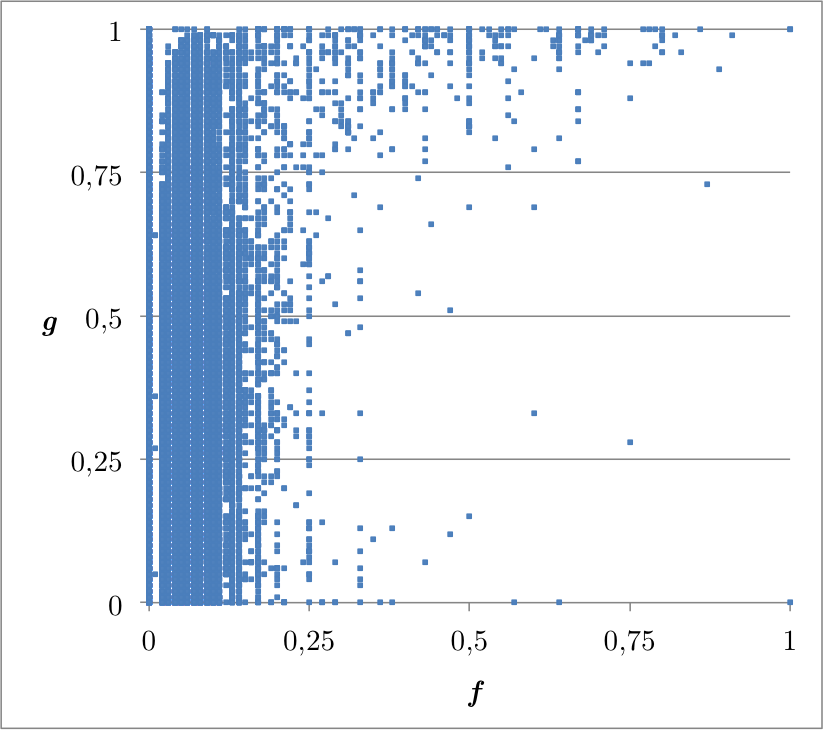
\includegraphics[width=8cm]{images/ap-staticvsdynamic/roassal.png}} \\[2cm] 
\subfloat[Fuel - $\rho_{f,g}=0,1176$]{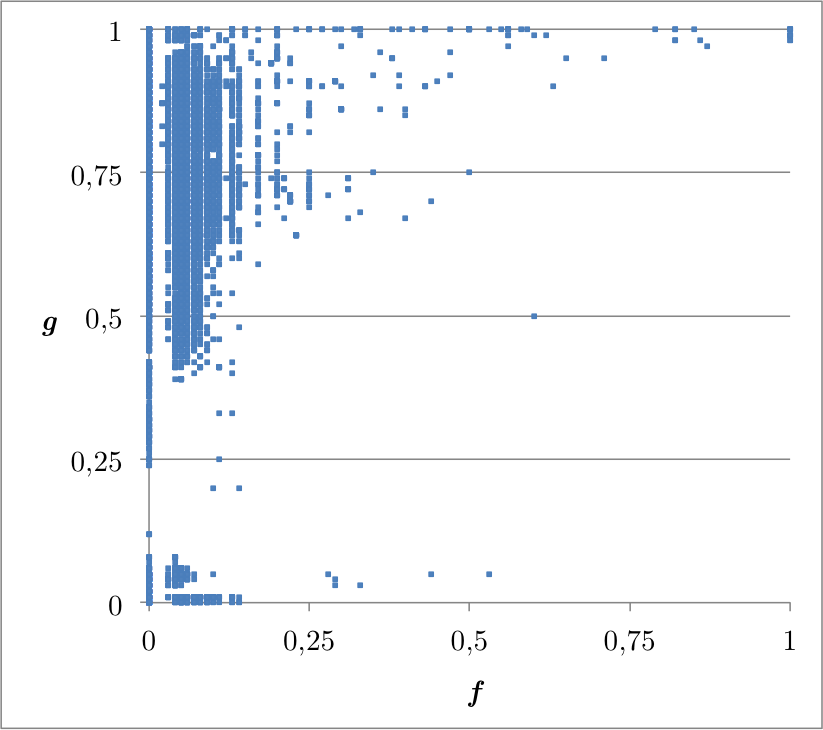
\includegraphics[width=8cm]{images/ap-staticvsdynamic/fuel.png}}
\end{tabular}
\caption{Resultados comparación de métricas $f$ y $g$}
\figlabel{ap-stat-dyn}
\end{figure}

\par Los graficos muestran que no existe correlación entre las dos métricas ya que en ninguno de los gráficos se ve alguna forma linear que lo indique. Esto último se ve reforzado cuando se toma en cuenta los valores del coeficiente de correlación de Pearson ($\rho_{f,g}$) de cada uno que son muy cercanos a cero, lo que indica que no existe correlación lineal entre las dos métricas.

\par Como consecuencia se puede deducir que dos tests con una gran porción de código duplicado no necesariamente tienen cubren los mismos métodos, o sea, no necesariamente testean la misma porción de código.

\par Se concluye que la duplicación de código entre tests no puede ser usado para inferir que son semánticamente similares. Por tanto, cualquier análisis comparativo entre tests debe hacerse considerando el código fuente y características de análsis estático, como también datos obtenidos durante su ejecución entre otros aspectos del análisis dinámico. 




%=====
%=====
%=====

% \par Para ilustrar lo anterior, se presenta el código de los tests: {\tt testAddingColoredElement} y {\tt testVisualizingBigClasses} 
% %=== Ejemplo
% \begin{codeWithLineNumbers}
% <i>testAddingColoredElement</i>
% 	canvas := ROView new.
% 	el1 := ROBox green element.
% 	el2 := ROBox red element.
% 	canvas add: el1; add: el2.
% 	self shouldnt: [ canvas open ] raise: Error

% <i>testVisualizingBigClasses</i>
% 	canvas := ROView new.
% 	Collection withAllSubclasses do: [ :cls |
% 		cls numberOfMethods > 10
% 			ifTrue: [ el := ROBox red element ]
% 			ifFalse: [ el := ROBox green element ].
% 		canvas add: el ].
% 	self shouldnt: [ canvas open ] raise: Error
% \end{codeWithLineNumbers}\codelabel{ejemplo-stat-dyn} 

% \par El código de {\tt testAddingColoredElement} crea un canvas (lienzo donde se dibujan los elementos gráficos) para posionar sobre esta una caja verde y otra roja. Por su parte, en {\tt testVisualizingBigClasses} se crea una visualizacion que representa algunas clases coloreadas según una condición particular. Cada subclase de {\tt Collection} está asociada a una caja. Si la clase tiene más de 10 métodos, la caja se pinta en rojo, de lo contrario en verde. 

% \par Los dos tests tienen un 95\% de metodos testeados en común, el 5\% que los diferencia se debe a algunos cachés están activados cuando el número de cajas excede cierto número límite. 

% \chapter{¿Por qué la cobertura no es suficiente para comparar dos tests?}\aplabel{pq-cobertura}

\par La cobertura de tests~\cite{Horwi02a} intenta determinar qué proporción de una parte de un programa es ejecutada durante el ciclo de pruebas. La cobertura de test se reporta comúnmente como la proporción de paquetes, clases, métodos y líneas de código fuente que fueron ejecutados por los tests. Revisar el código cubierto por los tests es una técnica efectiva para idenficar la porción de un software está asegurado por los tests. La medida tradicional de cobertura~\cite{Mock09a,Piwo93a} de test recae en marcar elementos estructurales del software tales como sentencias (o statements), métodos o clases que son cubiertos durante la ejecución.

\par Como sea la forma de marcar aquellos elementos, es igualmente útil para identificar y medir cual porción del código está siendo cubierta o no por los tests. Sin embargo, para conocer realmente si dos test están intentando testear lo mismo, diferenciarlos por lo su cobertura parece no ser suficiente~\cite{van2001refactoring,greiler2012test}.    

\par Para ilustrar lo anterior, se presenta el código de los tests: {\tt testAddingColoredElement} y {\tt testVisualizingBigClasses} :

%=== Ejemplo
\begin{codeWithLineNumbers}
<i>testAddingColoredElement</i>
	canvas := ROView new.
	el1 := ROBox green element.
	el2 := ROBox red element.
	canvas add: el1; add: el2.
	self shouldnt: [ canvas open ] raise: Error

<i>testVisualizingBigClasses</i>
	canvas := ROView new.
	Collection withAllSubclasses do: [ :cls |
		cls numberOfMethods > 10
			ifTrue: [ el := ROBox red element ]
			ifFalse: [ el := ROBox green element ].
		canvas add: el ].
	self shouldnt: [ canvas open ] raise: Error
\end{codeWithLineNumbers}\codelabel{ejemplo-stat-dyn} 

\par El código de {\tt testAddingColoredElement} crea un \emph{canvas} (lienzo donde se dibujan los elementos gráficos) para posionar sobre esta una caja verde y otra roja. Por su parte, en {\tt testVisualizingBigClasses} se crea una visualizacion que representa algunas clases coloreadas según una condición particular. Cada subclase de {\tt Collection} está asociada a una caja. Si la clase tiene más de 10 métodos, la caja se pinta en rojo, de lo contrario en verde. 

\par Los dos tests tienen un 95\% de metodos testeados en común, el 5\% que los diferencia se debe a algunos cachés que se activan cuando el número de cajas excede cierto número límite (este comportamiento no se muestra en el código presentado arriba). 

\par Aunque exista un solapamiento considerable desde el punto de vista de los métodos que cubren, estos dos tests no deberían ser considerados redundantes pues el escenario mostrado en cada uno tiene su propia relevancia y no son comparables. 

\par Por lo tanto, dos tests que son similares por su cobertura pueden ser semánticamente muy distintos. Esta diferencia semántica no es expresada por la cobertura y para revelarla se hace necesaria mayor información como por ejemplo más datos característicos de su ejecución e información experta por parte de los desarrolladores. 
% ---* APENDICE *---

\chapter{Distribución de Tests en Roassal}

\par A continuación se muestra la información sobre la distribución de los tests en los unit test de la versión 441 de Roassal.

\begin{table}[h] 
    \centering 
    \begin{tabular}{|l|c|c|}
    	\hline
        \textbf{\# de test} & \textbf{\# de unit test} & \textbf{\%} \\ \hline\hline
        $\left[ 0,5 \right]$	& 54	&68 \\ \hline
		$\left( 5,10 \right]$	& 13	&16	\\ \hline
		$\left( 10,15 \right]$	& 8	&10	\\ \hline
		$\left( 15,20 \right]$	& 1	&1	\\ \hline
		$\left( 20,50 \right]$	& 2	&3	\\ \hline
		$\left( 50,80 \right]$	& 1	&1	\\ \hline
		$\left( 80,100 \right]$ & 1 &1	\\ 	\hline \hline
		TOTAL	& 80	&100	\\ \hline
    \end{tabular}
    \caption{Distribución de los tests methods por unit test en Roassal}
    \tablabel{distribucion-tests}
\end{table} 

\large FALTA datos brutos
% ---* APENDICE *---

\chapter{Datos Exp. Clustering}





\end{document}
